\section{Implementation}

\subsection{Data Collection}

There is no historical data for bus arrival times available online, so all the data that I will use to train and test my models has to be manually collected. \\

The following bus routes were chosen to collect data from: 6, 7, 9, 14, 35, 37, 52, 69, 267, 277, 328, 452. Of these routes, the 6, 14, 37, 52 and 69 bus routes are twenty four hour bus routes and the 37, 69, 267 and 277 bus routes do not travel through Zone 1. This allows there to be variety in the travel routes, traffic conditions and times of travel and so the data collected is not heavily biased towards particular areas of London. There is also some overlap in stops between the bus routes, for example the 52 to Victoria and the 452 to Vauxhall have a 23 stop (and therefore, also route) overlap from "Station Terrace" to  "Knightsbridge Station /\ Harrods". This ensures information on journey times between stops doesn't rely on data from just one bus route. \\

\textbf{1) Call Countdown API}: The JSON information returned from the Countdown call is converted into a list of dictionaries, where each dictionary represents a single vehicle. The format of each dictionary is as below:

\begin{lstlisting}
    vehicle_info = {
                "vehicle_id": vehicle_id,
                "bus_stop_id": bus_stop_id,
                "direction": direction,
                "expected_arrival": eta,
                "time_of_req": time_of_request
            }
\end{lstlisting}

In the dictionary, the \texttt{vehicle\_id}, \texttt{bus\_stop\_id} and \texttt{direction} are strings and the \texttt{expected\_arrival} and \texttt{time\_of\_req} are Python \texttt{Datetime} objects. \\

\textbf{2) Update the estimated arrival time of a bus}: For each of the dictionaries, check if the vehicle corresponds to one already in the \texttt{bus\_information\_route} table. If it already exists, then update its expected arrival time, otherwise, it is a new vehicle to track and so needs to be added to the table. \\

\textbf{3) Check if the bus has arrived or not}:  If the current time is after the predicted arrival time of the bus, then it is classified as 'due'. If the current time is 5 minutes after the predicted arrival time of the bus, then it is classified as 'arrived'. Return the 'due' and 'arrived' vehicles in separate lists so that they can be processed and written to the correct database. \\

\textbf{4) Write to the relevant database}: The `due' buses have updated arrival times. Therefore, this information is updated in the \texttt{bus\_information\_route} table. The 'arrived' buses are removed from the \texttt{bus\_information\_route} table and added to the \texttt{bus\_arrivals\_route} table. When adding to the \texttt{bus\_arrivals\_route} table, check to see if on this day this particular vehicle is already in the table. It is necessary to check this because each vehicle will complete the bus route more than once per day, and therefore, the current trip number has to be kept track of too. This trip number is appended to the end of the \texttt{vehicle\_id}.

\subsection{Historical Models}

According to the eight sub-models described in Section \ref{section:historical-model-design}, the journey times were calculated for random pairs of stops and routes. The weighted average was then calculated, using the pre-discovered weightings. Using \texttt{sklearn}'s inbuilt functions, the mean absolute error (MAE) and root mean square error (RMSE) were calculated, first for journeys that are five stops apart. The best two sub-models that obtained the best combined RMSE and MAE were then tested using stops that are further apart. 

\subsection{Regression Models}

The data collected from the tables is in the following format as shown in Figure \ref{fig:regression-databefore}. It must be processed into the format as shown in Figure \ref{fig:regression-datamiddle} in order for it to be able to be analysed.

\begin{figure}[H]
\begin{center}
    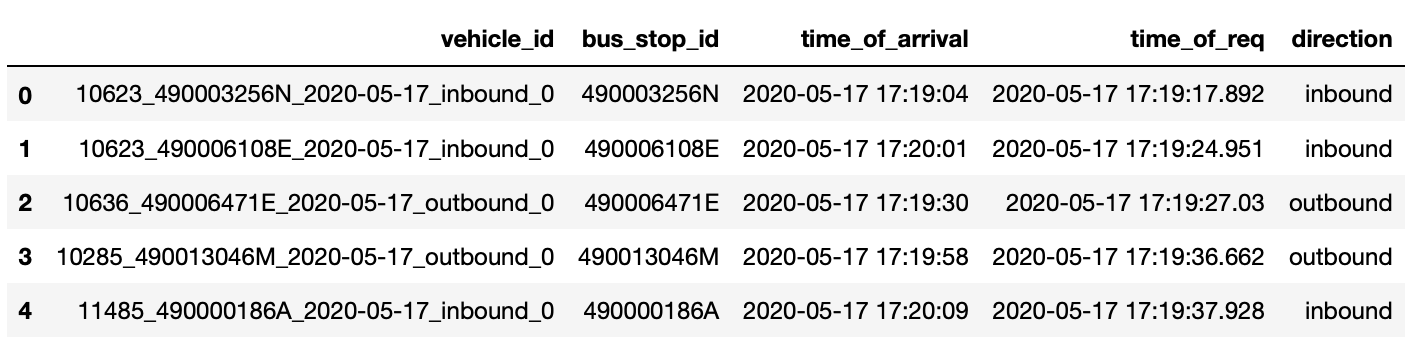
\includegraphics[keepaspectratio, width=15cm]{Images/regression-databefore.png}
    \caption{Data before}
    \label{fig:regression-databefore}
\end{center}
\end{figure}

The data collected has the time of arrival of a bus at a stop on a route, but it does not have the journey time since this would require it to be given a start and end stop. Therefore, pairs of stops across the routes were chosen to form journey routes. The pairs of stops were chosen so that there was variety in the gap sizes between the stops. The routes were also chosen so that there would be 24-hour bus routes as well as bus routes that don't run through Zone 1. The journey times were then put into a dataframe. \\

For each journey collected, the code looks at the time of arrival and converts the date into a day of week using Python's \texttt{calendar} library. Then, it converts this day of week into either a weekday or weekend. The code then checks if the time of arrival was between March 24th 2020 and 31st May 2020 or not. If it was in between those dates, then it categorises the entry as being during lockdown, else as pre/post-lockdown. The code also looks at the hour at which the bus arrives at the destination stop. This hour counted as the time of day of the journey. The resulting dataframe can be seen in Figure \ref{fig:regression-datamiddle}.

\begin{figure}[H]
\begin{center}
    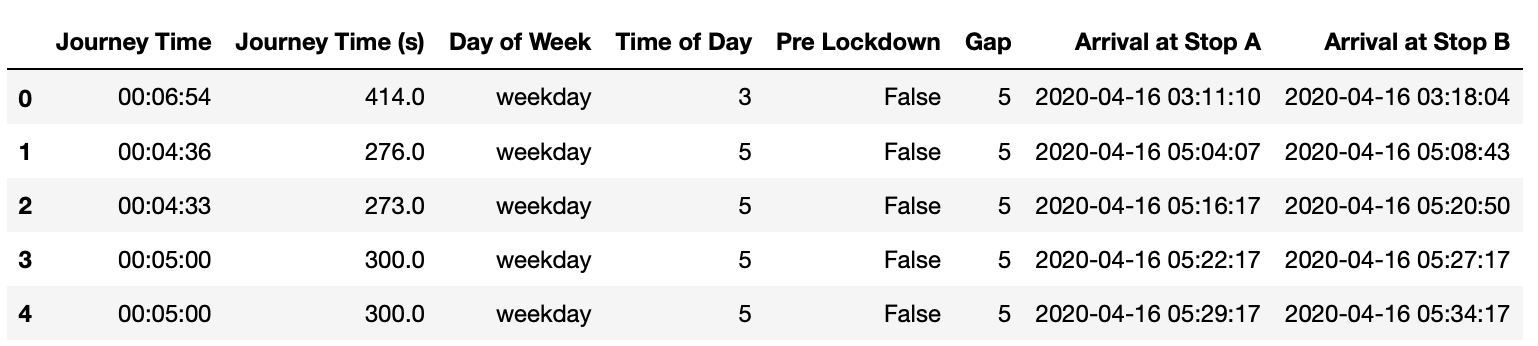
\includegraphics[keepaspectratio, width=15cm]{Images/regression-datamiddle.png}
    \caption{dataframe of processed data}
    \label{fig:regression-datamiddle}
\end{center}
\end{figure}

Figure \ref{fig:regression-pairplot} shows a pair plot of the training data where the possible factors are plotted against each other alongside their Pearson correlation coefficient.

\begin{figure}[H]
\begin{center}
    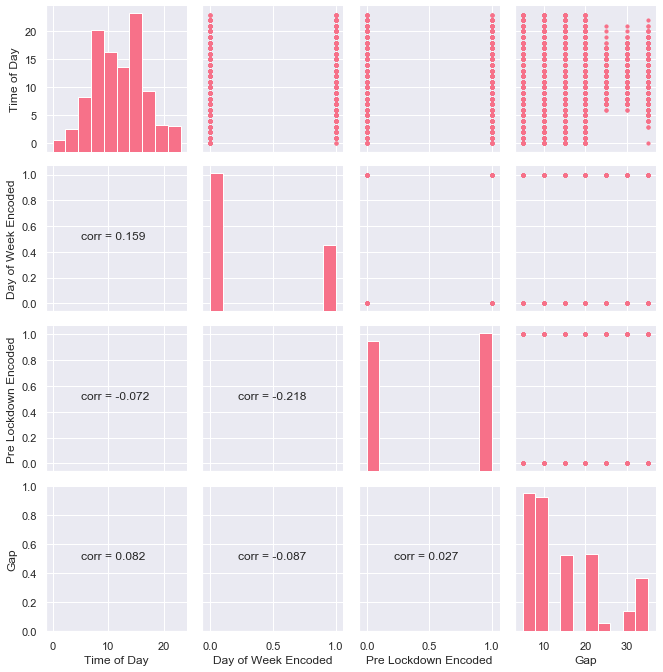
\includegraphics[keepaspectratio, width=12cm]{Images/regression-pairplot.png}
    \caption{Feature Pairplot}
    \label{fig:regression-pairplot}
\end{center}
\end{figure}

It can be seen from Figure \ref{fig:regression-pairplot} that the correlation coefficients are very close to 0. This implies that these features are indeed independent of each other and can therefore be used together in multivariate regression. \\

Figure \ref{fig:regression-pairplot} indicates that there was more data collected on weekdays versus weekends (as can be seen from the 2nd graph along the major diagonal - where 0 is the weekday and 1 is the weekend). From the top left graph it can be seen that for stops that are between 20 to 30 stops apart, there are gaps in the data collected. For example, it can be seen that approximately between 00:00 to 05:00 there is no data for journeys between stops that are 25 stops apart.\\

\textbf{1) Calculate `global' prediction}: Before the data can be fed into a regression or interpolation model, the values must be encoded. So, using \texttt{sklearn}'s label encoder, the day of week and pre-lockdown are converted into categorical values. Based on Equation \ref{eq:part1-regression}, the time of day has to be one-hot encoded, so this is also done using \texttt{sklearn}. The result of this can be seen in Figure \ref{fig:regression-dataforregression}. 

\begin{figure}[H]
\begin{center}
    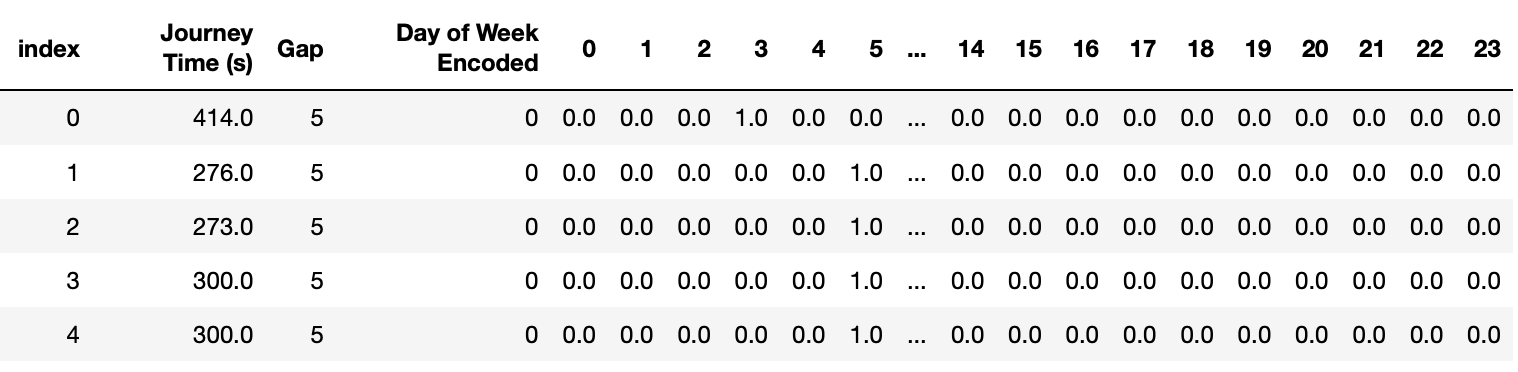
\includegraphics[keepaspectratio, width=15cm]{Images/regression-input.png}
    \caption{Data for part 1 regression}
    \label{fig:regression-dataforregression}
\end{center}
\end{figure}

The features are scaled and then fed into a linear regression model for training. \\

\textbf{2) Calculate `local' prediction}: For the three sub-models, it is necessary to get the last 10 journeys for each request time and pair of stops, as well as how long ago the journey was in relation to the journey time. An example can be seen in Figure \ref{fig:regression-part2}, where `Bus 0' is the most recent bus to have completed the journey and `Bus 0 time to req' is how long ago in seconds this bus completed that journey relative to the request time. The columns go all the way down to `Bus 9' and `Bus 9 time to req'.

\begin{figure}[H]
\begin{center}
    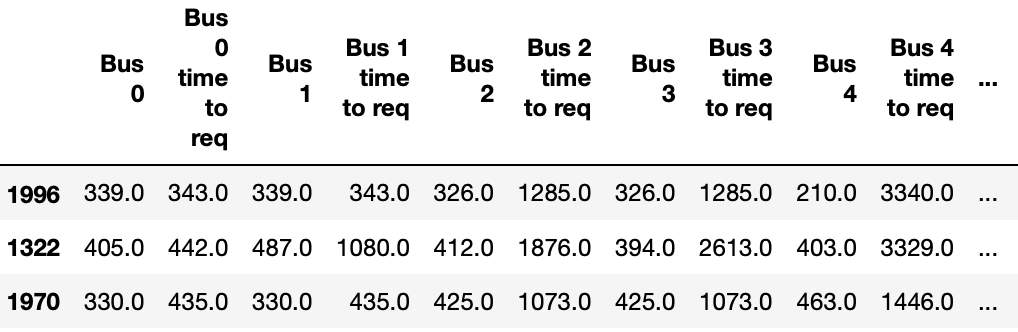
\includegraphics[keepaspectratio, width=14cm]{Images/regression-datapart2.png}
    \caption{Data for part 2 sub-model}
    \label{fig:regression-part2}
\end{center}
\end{figure}

\subsection{Phone App}

TODO 

\clearpage